\documentclass[10pt]{article}
\usepackage{itcep, stmaryrd, tikz, pgflibraryplotmarks, multicol, pgfplots}
\usepackage[margin=1in, nohead, pdftex]{geometry}

\topmargin -0.2in
\pagestyle{empty}
\singlespacing
\let\oldhat\hat
\renewcommand{\vec}[1]{\mathbf{#1}}
\renewcommand{\hat}[1]{\oldhat{\mathbf{#1}}}

\definecolor{light-gray}{gray}{0.95}
\newcommand{\code}[1]{\colorbox{light-gray}{\texttt{#1}}}

\newcommand{\headerclass}{Machine Learning Camp}
\newcommand{\headersection}{Day 2: Introduction to Classification}
\newcommand{\headertitle}{Iris Flower Dataset}

\def\C{\mathbb{C}}
\def\R{\mathbb{R}}
\parindent 0ex
\begin{document}
%==================================================================================================================================================
\headerclass\xspace \hspace{\stretch{1}} \headersection\\
\begin{center}{ \large \textbf{\headertitle} }\end{center}
%==================================================================================================================================================

To practice using the $k$-nearest neighbor algorithm in python, we'll be using a very famous dataset, the \emph{Iris flower data set} from statistician and biologist Ronald Fisher in 1936. This dataset consists of measurements taken from 150 iris flowers from three different iris species, Iris setosa, Iris virginica, and Iris versicolor. Four features were measured for each flower sample: sepal length, sepal width, petal length, and petal width.\\

\begin{minipage}{.5\textwidth}
\begin{center}
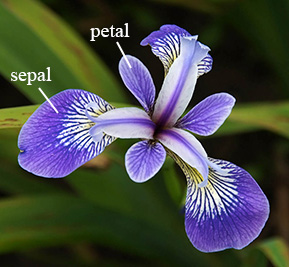
\includegraphics[height = 1.5in]{iris_with_labels}
\end{center}
\end{minipage}
\begin{minipage}{.5\textwidth}
The \emph{petals} are the colorful leaves of a flower, which surround the reproductive parts of the flower.\\

The \emph{sepals} are outside of the petals, and they protect the flower while it's in bud. When the flower blooms, the sepals support the petals. In most flowers, the sepals are green, but for these irises, the sepals are purple.
\end{minipage}\\

When Fisher first introduced the iris data set, he showed how a machine learning method called \emph{linear discriminant analysis} can be used for classification of these iris species. Since then, the Iris dataset has become one of the most commonly used datasets for practicing, testing, and demonstrating machine learning classification algorithms. As you continue to study machine learning, you're likely to come across the iris dataset again and again!


\end{document}
